\documentclass[12pt]{article}
	
\title{CSC 320 - Worksheet 0}
\author{Nadeem Abdul Hamid}
\date{January 9, 2024}  


\usepackage[margin=1in]{geometry}		% For setting margins
\usepackage{amsmath}				% For Math
\usepackage{amsthm}
\usepackage{fancyhdr}				% For fancy header/footer
\usepackage{graphicx}				% For including figure/image
\usepackage{cancel}					% To use the slash to cancel out stuff in work
\usepackage[shortlabels]{enumitem}
\usepackage{hyperref}
\usepackage{jigsaw}

\usepackage{algorithm,caption}
\usepackage{algpseudocodex}
% docs: https://ctan.math.washington.edu/tex-archive/macros/latex/contrib/algpseudocodex/algpseudocodex.pdf


%%%%%%%%%%%%%%%%%%%%%%
% Set up fancy header/footer
% taken from https://www.overleaf.com/latex/templates/homework-template/yvgnmrbywwnp
\makeatletter    % for \@ in \@title
\pagestyle{fancy}
\fancyhead[LO,L]{\@author}
\fancyhead[CO,C]{\@title}
\fancyhead[RO,R]{\@date}
\fancyfoot[LO,L]{}
\fancyfoot[CO,C]{\thepage}
\fancyfoot[RO,R]{}
\renewcommand{\headrulewidth}{0.4pt}
\renewcommand{\footrulewidth}{0.4pt}
\makeatother    % restore
%%%%%%%%%%%%%%%%%%%%%%


%%%%%%%%%%%%%%%%%%%%%%
% from: https://tex.stackexchange.com/questions/14667/does-latex-define-a-semantic-equivalent-of-textbf
\makeatletter
\newcommand{\strong}[1]{\@strong{#1}}
\newcommand{\@@strong}[1]{\textbf{\let\@strong\@@@strong#1}}
\newcommand{\@@@strong}[1]{\textnormal{\let\@strong\@@strong#1}}
\let\@strong\@@strong
\makeatother
%%%%%%%%%%%%%%%%%%%%%%


\newcommand{\emptybox}[2][\textwidth]{%
  \begingroup
  \setlength{\fboxsep}{-\fboxrule}%
  \noindent\framebox[#1]{\rule{0pt}{#2}}%
  \endgroup
}

\newtheorem{theorem}{Theorem}
\newtheorem{lemma}{Lemma}

\usepackage{verse}

\begin{document}

\section{Algorithm Design \& Analysis Process}

Fill in the flowchart below with the appropriate process in each box.

\begin{table}[h]
\begin{tabular}{|l|}
    \hline
    Design an algorithm.\\
    Analyze the running time.\\
    Prove correctness.\\
    Understand and clearly specify the problem.\\
    Implement (code) the algorithm.\\
    \hline
\end{tabular}
\end{table}
    
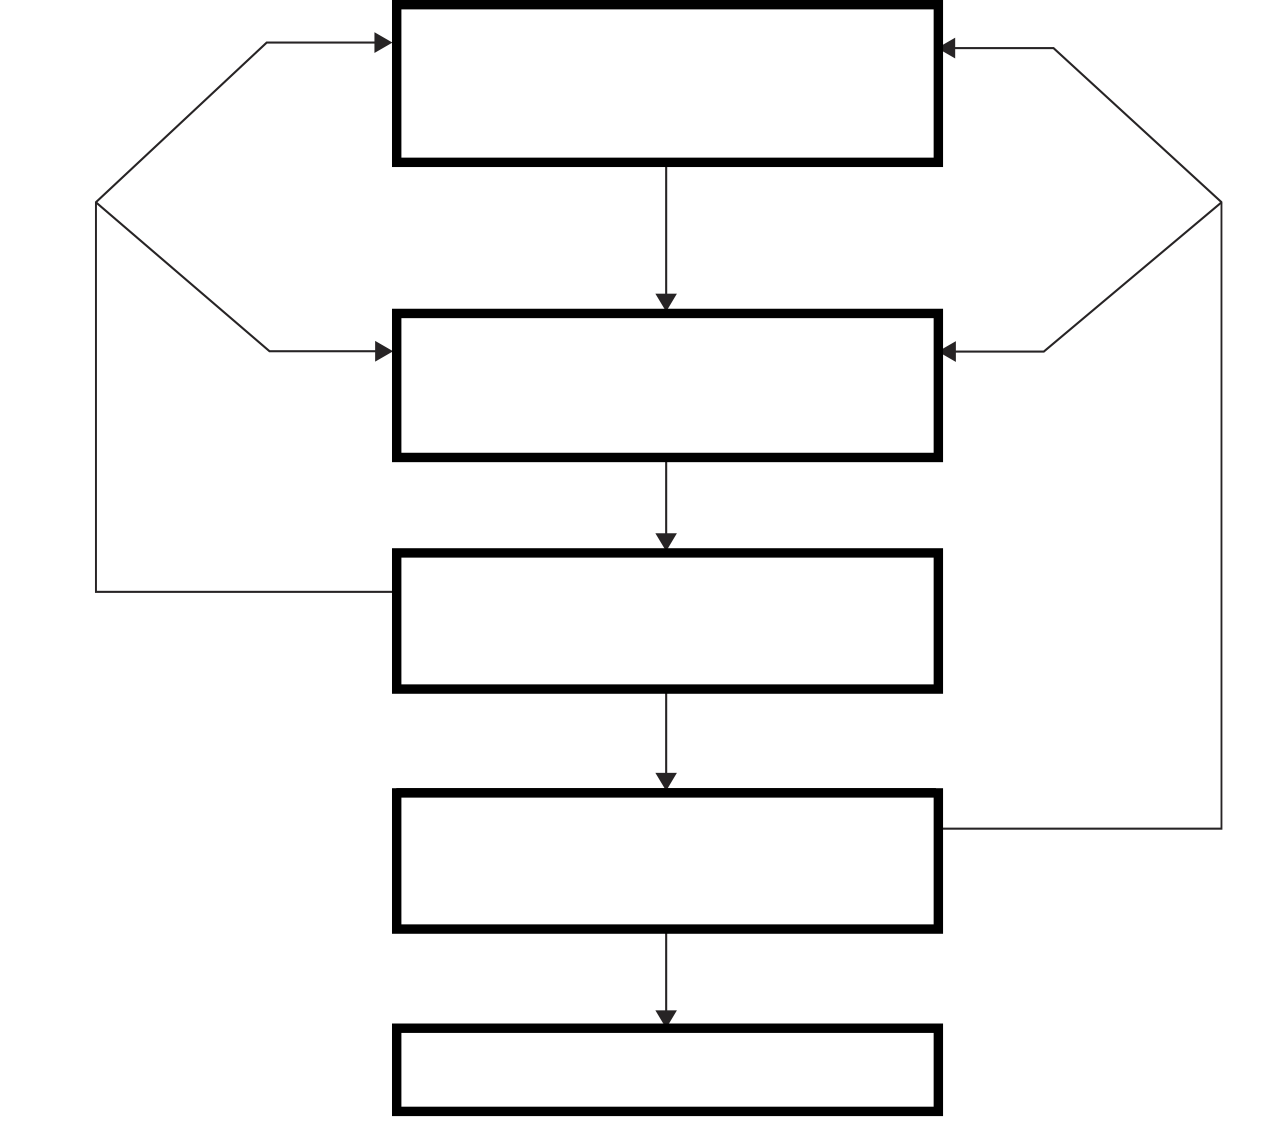
\includegraphics[width=.75\linewidth]{w00-flowchart.png}


\clearpage
\section{Writing Pseudocode}

Consider the following cumulative variation of a popular children's song:

\vspace{1em}
\framebox{  
    \begin{minipage}{\textwidth}
    \begin{verse}
        \begin{altverse}
        Old MacDonald had a farm. E-I-E-I-O.\\
        And on that farm he had a \strong{pig}.\\
        With an \strong{oink oink} here. And an \strong{oink oink} there.\\
        Old MacDonald had a farm. E-I-E-I-O.
        \end{altverse}

        \begin{altverse}
        Old MacDonald had a farm. E-I-E-I-O.\\
        And on that farm he had a \strong{duck}.\\
        With an \strong{quack quack} here. And an \strong{quack quack} there.\\
        With an oink oink here. And an oink oink there.\\
        Old MacDonald had a farm. E-I-E-I-O.
        \end{altverse}

        \begin{altverse}
        Old MacDonald had a farm. E-I-E-I-O.\\
        And on that farm he had a \strong{horse}.\\
        With an \strong{neigh neigh} here. And an \strong{neigh neigh} there.\\
        With an {quack quack} here. And an {quack quack} there.\\
        With an oink oink here. And an oink oink there.\\
        Old MacDonald had a farm. E-I-E-I-O.
        \end{altverse}

        \begin{altverse}
        Old MacDonald had a farm. E-I-E-I-O.\\
        And on that farm he had a \strong{sheep}.\\
        With an \strong{baaa baaa} here. And an \strong{baaa baaa} there.\\
        With an {neigh neigh} here. And an {neigh neigh} there.\\
        With an {quack quack} here. And an {quack quack} there.\\
        With an oink oink here. And an oink oink there.\\
        Old MacDonald had a farm. E-I-E-I-O.
        \end{altverse}

        \begin{altverse}
        ~\vdots
        \end{altverse}
    \end{verse}    
\end{minipage}}\vspace{1em}

Write pseudocode for an algorithm to sing this song, given lists of animals and sounds:

\begin{algorithm}
    \caption{Farm Song Algorithm}
    \label{alg:farmsong}
    \begin{algorithmic}
        \Procedure{FarmSong}{$\textit{animals}[1..n], \textit{sounds}[1..n]$}

        \LComment{Fill this in\vspace{1.2in}\\}

        \EndProcedure
    \end{algorithmic}
\end{algorithm}


\clearpage
\section{Understanding Algorithms}

Let's figure out what the following algorithm does:

\begin{algorithm}
    \caption{Unknown Algorithm}
    \label{alg:unknown}
    \begin{algorithmic}
        \Procedure{Something}{$A[1..n]$}
        \LComment{Input: Array $A[1..n]$ of numbers\\
                  Output: ??? }
        \State $d \gets \infty$
        \For{$i = 1, \dots, n$}
            \For{$j = 1, \dots, n$}
                \If{$i \neq j$ \strong{and} $|A[i] - A[j]| < d$}
                    \State $d \gets |A[i] - A[j]|$
                \EndIf
            \EndFor
        \EndFor
        \State \Return $d$
        \EndProcedure
    \end{algorithmic}
\end{algorithm}

\begin{enumerate}
    \item Write down a small sample array, $A$.
    \item Trace through the execution of the nested loops.
    \item What is the \textbf{if} statement checking? 
    \item How many times is $d$ updated for your array?
    \item What does the algorithm produce as the overall result?
\end{enumerate}


\clearpage
\section{Reformulating Algorithms}

Consider the following iterative\footnote{``Iterative'' means it is described using a \emph{loop} construct (\texttt{while} or \texttt{for}).} algorithm from the zeroth chapter of our textbook:

\begin{algorithm}
    \caption{Peasant multiplication}
    \label{alg:peasant}
    \begin{algorithmic}
        \Procedure{PeasantMult}{$x, y$}
        \State $prod \gets 0$
        \While{$x > 0$}
            \If{$x$ is odd}
                \State $prod \gets prod + y$
            \EndIf
            \State $x \gets \lfloor{x / 2}\rfloor$
            \State $y \gets y + y$
        \EndWhile
        \State \Return $prod$
        \EndProcedure
    \end{algorithmic}
\end{algorithm}

\begin{enumerate}
    \item Pick two 3-digit numbers and trace the execution of the algorithm on them.
    \item Why does the algorithm work?
    \item Rewrite the algorithm so that it is \emph{recursive} instead of iterative.
    \item How would you go about analyzing the running time of the algorithm?
\end{enumerate}



\clearpage
\section{Problem Types}

Let's talk about the most important/common types of problems encountered in CS.

\begin{table}[h]
    \caption{7 types of problems}
    \begin{tabular}{|c|c|c|c|}
        \hline
        Geometric problems & String processing & Sorting & Numerical problems \\
        \hline
        Searching & Combinatorial problems & Graph problems & \\
        \hline
    \end{tabular}
\end{table}

\begin{table}[h]
    \caption{Examples of applications}
    \begin{tabular}{|l|}
        \hline
        Find is the best route between two cities.\\\hline
        Find the closest pair among $n$ points in the plane. \\\hline
        Search an entire gene sequence for a particular subsequence of characters. \\\hline
        Rank Internet search results. \\\hline
        Compute the roots of a polynomial function. \\\hline
        Retrieve information from a large database. \\\hline
        Find a subset of numbers in a list that sum to zero. \\\hline
    \end{tabular}
\end{table}

Match up the seven problem types above, and the applications, with the definitions below:\\

%\begin{table}[h]
    \begin{tabular}{|c|l|c|}
        \hline
        Type & Description & Example \\\hline
        \hspace{1.25in} & Rearrange the items of a list in some order. & \hspace{1.5in} \\& & \\
        & & \\\hline
        & Finding a key in a set of data. & \\& & \\
        & & \\\hline
        & Handling a sequence of characters & \\
        & from an alphabet. &\\& & \\\hline
        & Modeling and analyzing a collection of  & \\
        & vertices connected by edges. &  \\& & \\\hline
        & Finding an object of a finite collection & \\
        & that satisfies certain constraints & \\& & \\\hline
        & Deal with objects such as points, lines, & \\
        & and polygons. & \\& & \\\hline
        & Problems that involve mathematical & \\
        & objects of continuous nature. & \\& & \\\hline
    \end{tabular}
%\end{table}



\end{document}  